\documentclass[utf8, xcolor=dvipsnames]{beamer}
% \usetheme{Frankfurt} % Boadilla - Ilmenau

\usepackage{graphicx}
\usepackage{setspace}
\usepackage{csquotes}
\usepackage{changepage}
\usepackage{color}
\usepackage[colorlinks = TRUE, allcolors = blue]{hyperref}
\useinnertheme{rectangles}
\usepackage{tikz}
\usetikzlibrary{graphs}
\usetikzlibrary{decorations.pathreplacing}

% \setbeamercovered{transparent}
\setbeamercolor{title}{bg=Blue, fg=white}
\setbeamercolor{title_int}{bg=white, fg=Blue}
\setbeamertemplate{navigation symbols}{}
\setbeamertemplate{itemize items}[circle]
\setbeamertemplate{blocks}[default]
\setbeamertemplate{headline}[default]
\setbeamertemplate{section in head}{}
\setbeamertemplate{subsection in head}{}
\setbeamercolor{section in foot}{fg=Blue, bg=white}
\setbeamercolor{subsection in foot}{fg=Blue, bg=white}
\setbeamercolor{frametitle}{fg=Blue, bg=white}
\setbeamercolor{footlinecolor}{bg=white,fg=Blue}
\useoutertheme[compress]{miniframes}

\makeatother
\setbeamertemplate{footline}
{%
  \leavevmode%
  \hbox{
  \begin{beamercolorbox}[wd=\paperwidth,ht=2.5ex,dp=1.125ex,leftskip=.3cm,rightskip=.3cm plus1fil]{footlinecolor}%
    \usebeamerfont{author in head/foot}
    \insertshorttitle\hfill\insertshortauthor\hfill\insertshortdate\hfill\insertframenumber/\inserttotalframenumber
  \end{beamercolorbox}}%
  \vskip0pt%
}
\setbeamertemplate{headline}[default]
{%
    \def\beamer@entrycode{\vspace*{0pt}}
}
\makeatletter

\title[Rebel groups]{Rebel groups and wartime governance}
\author[Francisco Villamil]{Francisco Villamil}
\date[UC3M / Fall 2022]{War, peace, and political violence\\Fall 2022\\Universidad Carlos III de Madrid}

\begin{document}


\begin{frame}
  \titlepage
\end{frame}


% ----------------------------------------------------
\begin{frame}
\frametitle{The universe of civil wars}
\centering

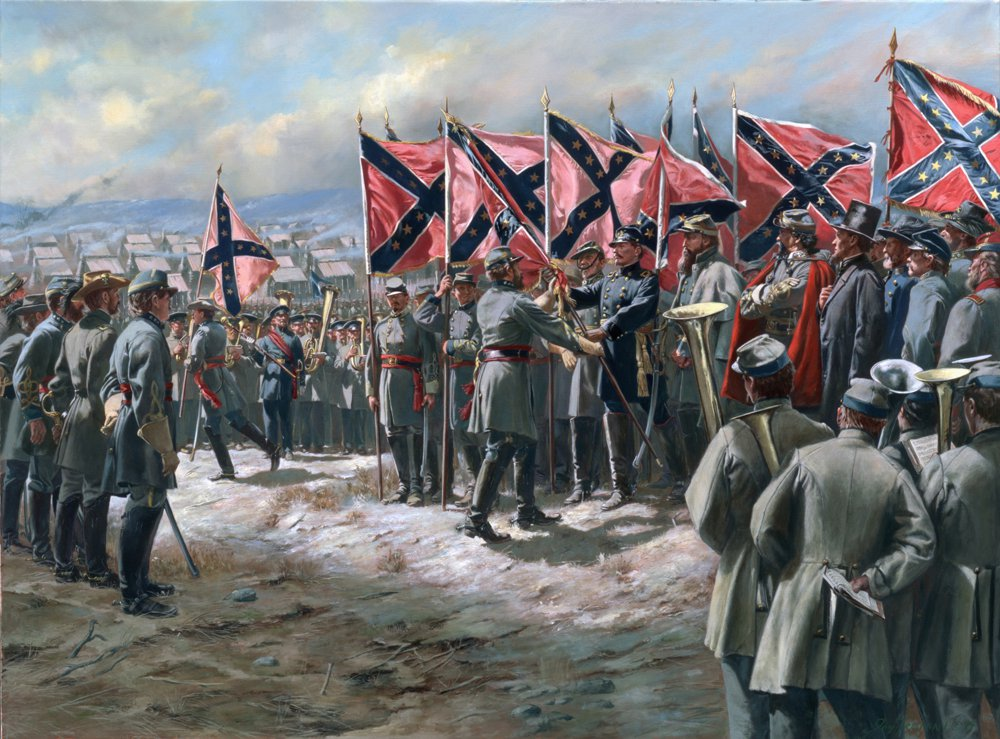
\includegraphics[width = 0.8\textwidth]{img/confederate}

\vspace{15pt}

Confederate Army (American Civil War)

\end{frame}
% ----------------------------------------------------

% ----------------------------------------------------
\begin{frame}
\frametitle{The universe of civil wars}
\centering

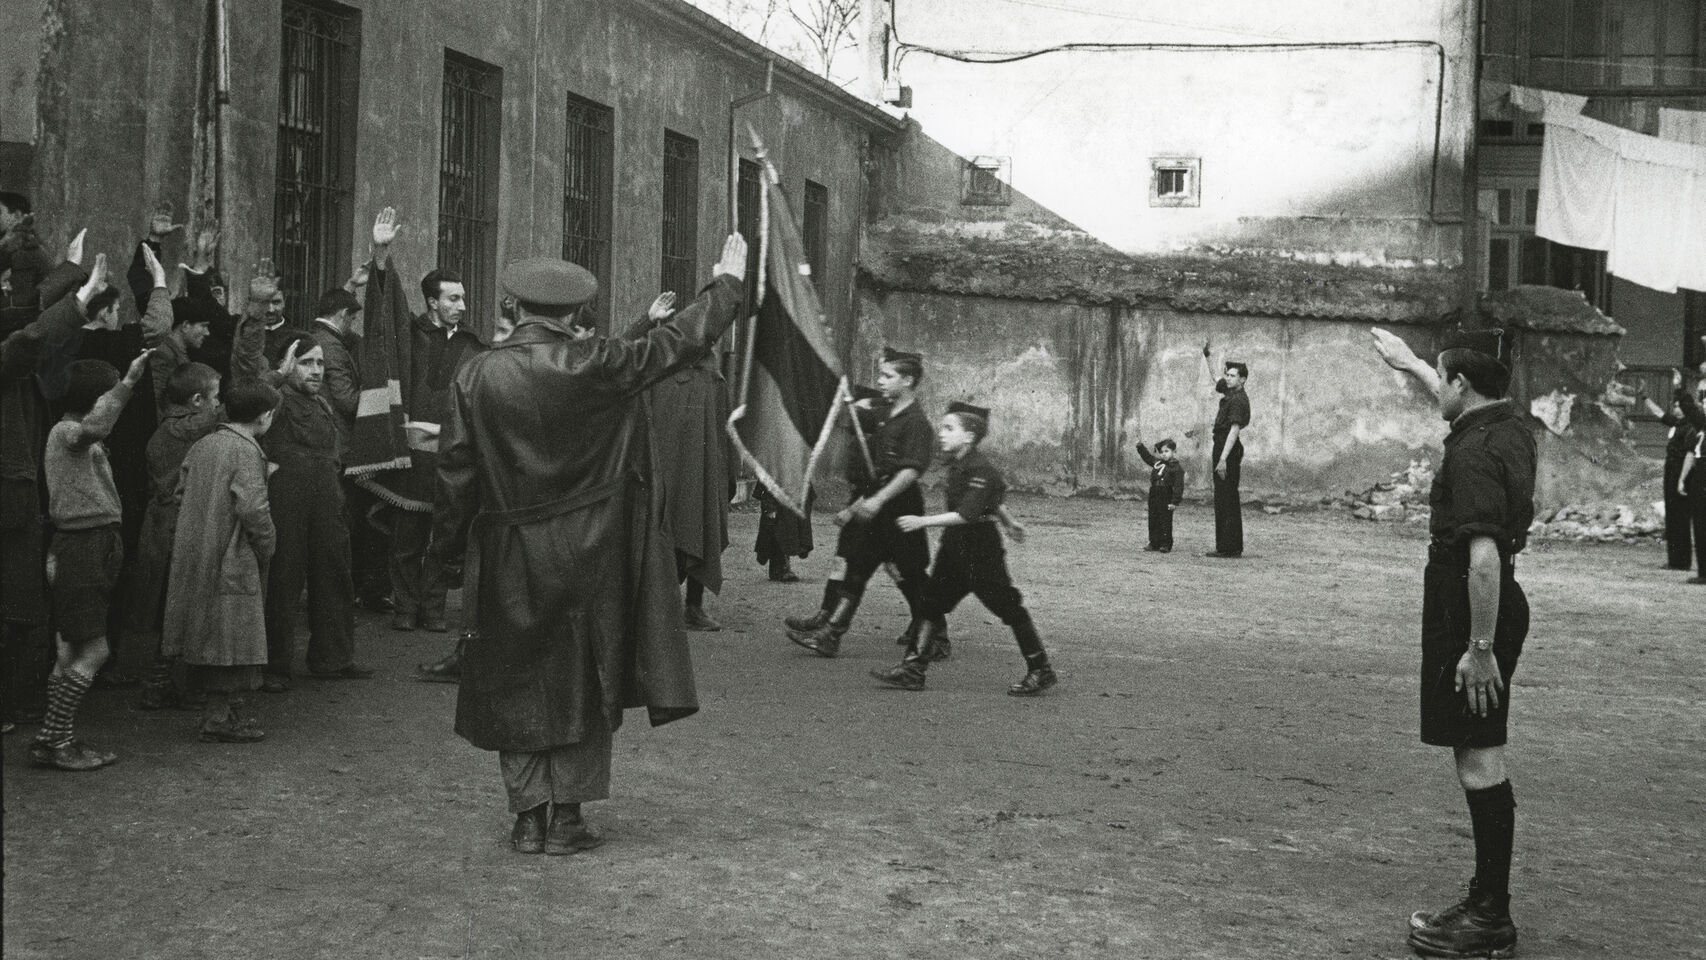
\includegraphics[width = 0.9\textwidth]{img/gv_oviedo}

\vspace{15pt}

Oviedo, 1937 (Spanish Civil War)

\end{frame}
% ----------------------------------------------------

% ----------------------------------------------------
\begin{frame}
\frametitle{The universe of civil wars}
\centering

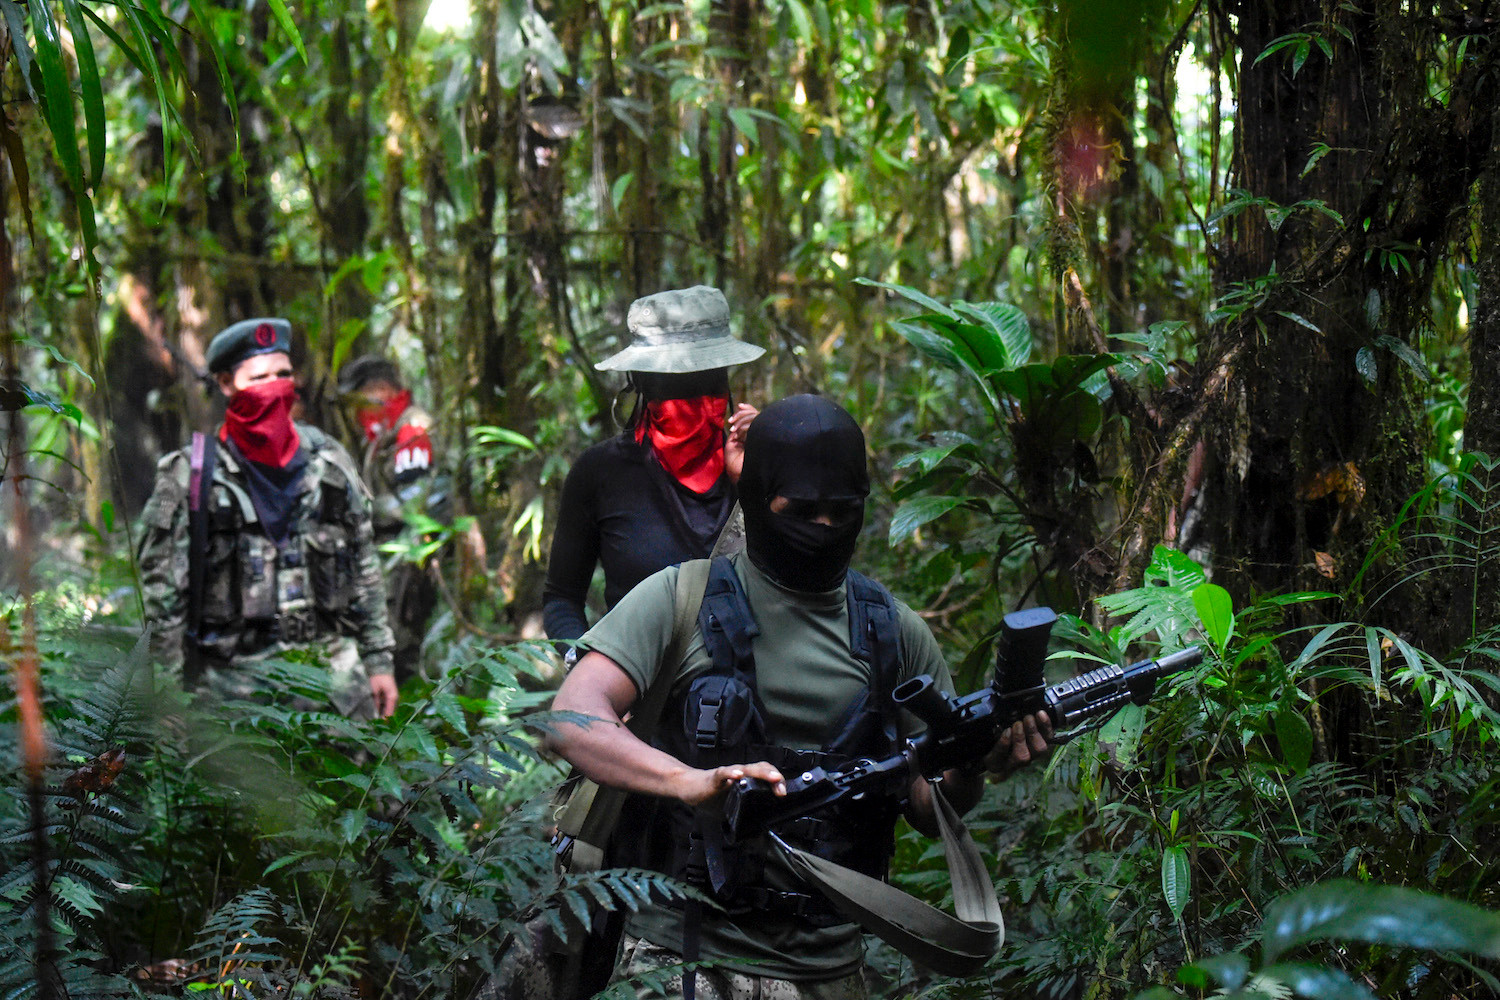
\includegraphics[width = 0.9\textwidth]{img/colombia}

\vspace{15pt}

ELN guerrilla (Colombian Civil War)

\end{frame}
% ----------------------------------------------------

% ----------------------------------------------------
\begin{frame}
\frametitle{The universe of civil wars}
\centering

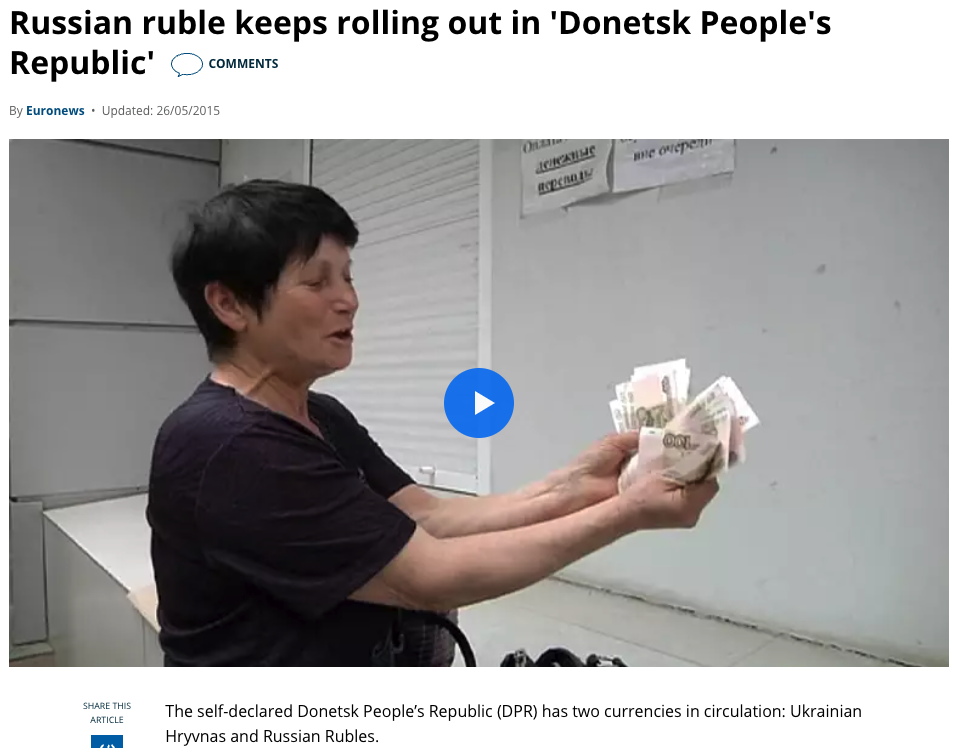
\includegraphics[width = \textwidth]{img/donbas}

\vspace{15pt}

Donetsk People's Republic

\end{frame}
% ----------------------------------------------------

% ----------------------------------------------------
\begin{frame}
\frametitle{The universe of civil wars}
\centering

\begin{itemize}
  \item We've seen this many times already: huge differences between civil wars
  \item Why?
\end{itemize}

\end{frame}
% ----------------------------------------------------

% ----------------------------------------------------
\begin{frame}
\frametitle{The universe of civil wars}
\centering

\begin{itemize}[<+->]
  \item<1-> Much of this variation is due to differences in rebel groups
  \begin{itemize}
    \item All states usually share some characteristics
  \end{itemize}
  \item<2-> What questions should interest us? (What's there to explain?)
  % \item Actions
  % \item Formation
  % \item Transformation
\end{itemize}

\end{frame}
% ----------------------------------------------------

% ----------------------------------------------------
\begin{frame}
\frametitle{The universe of civil wars}
\centering

\begin{itemize}
  \item<1-> Many differences in the way a civil war is fought
  \begin{itemize}
    \item Technology of rebellion: conventional wars, irregular wars, etc
    \item Recruitment patterns: who joins a rebel group and why?
    \item Patterns of violence: violence against civilians, etc
  \end{itemize}
  \item<2-> One more important aspect: wartime governance of civilians
  \begin{itemize}
    \item Whether and how rebel groups interact with local civilians
    \item Not directly related to warfare
    \item Not talking about violence here (only, at least)
  \end{itemize}
\end{itemize}

\end{frame}
% ----------------------------------------------------

% ----------------------------------------------------
\begin{frame}
\frametitle{Rebel governance}
\centering

\begin{itemize}
  \item<1-> Wars are not continuous and non-stop violence and anarchy
  \item<2-> Rebels make a decision on how to rule local civilians
  \item<2-> Civilians also have some influence on how they are ruled
  \item<3-> This `wartime social order' can be purely coercive and violent, but most groups engage in some form of governance: taxation, popular assemblies, courts, schools, etc
\end{itemize}

\end{frame}
% ----------------------------------------------------

% ----------------------------------------------------
\begin{frame}
\frametitle{Sri Lankan civil war (1983--2009)}
\centering

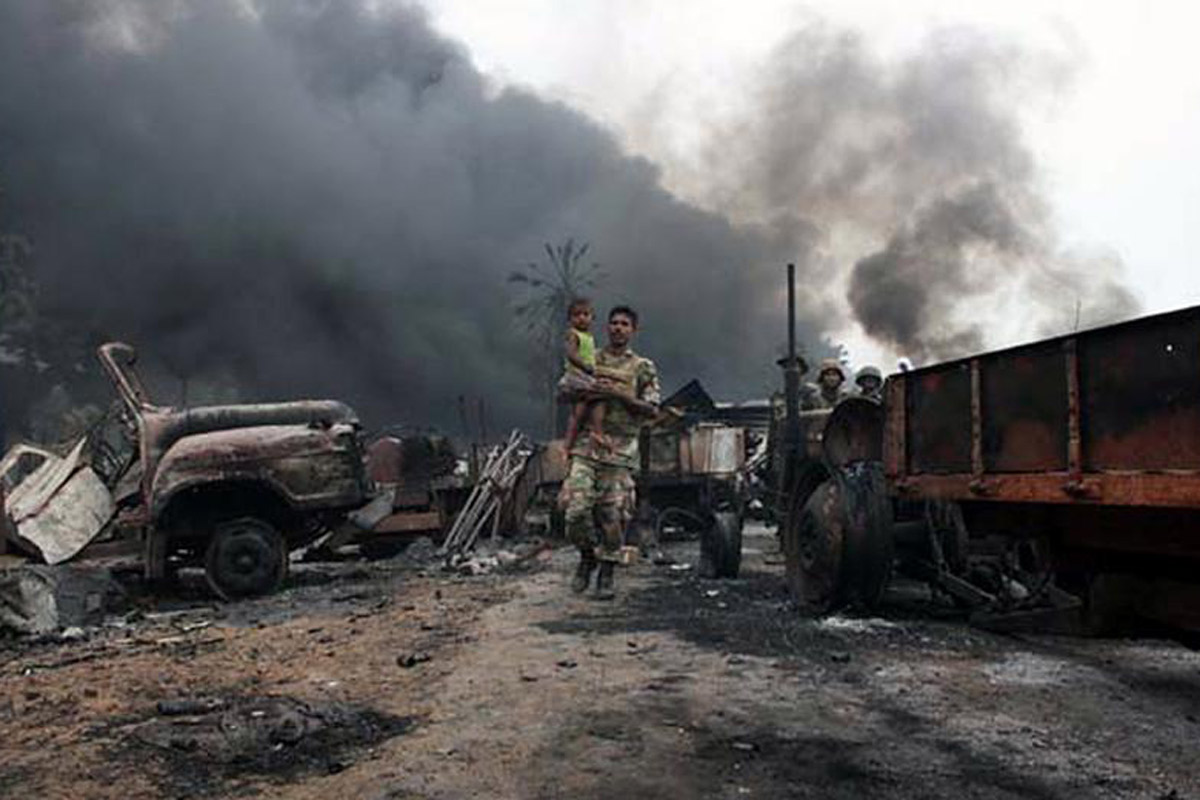
\includegraphics[width = 0.8\textwidth]{img/sri_lanka_war}

\end{frame}
% ----------------------------------------------------

% ----------------------------------------------------
\begin{frame}
\frametitle{LTTE (Liberation Tigers of Tamil Eelam)}
\centering

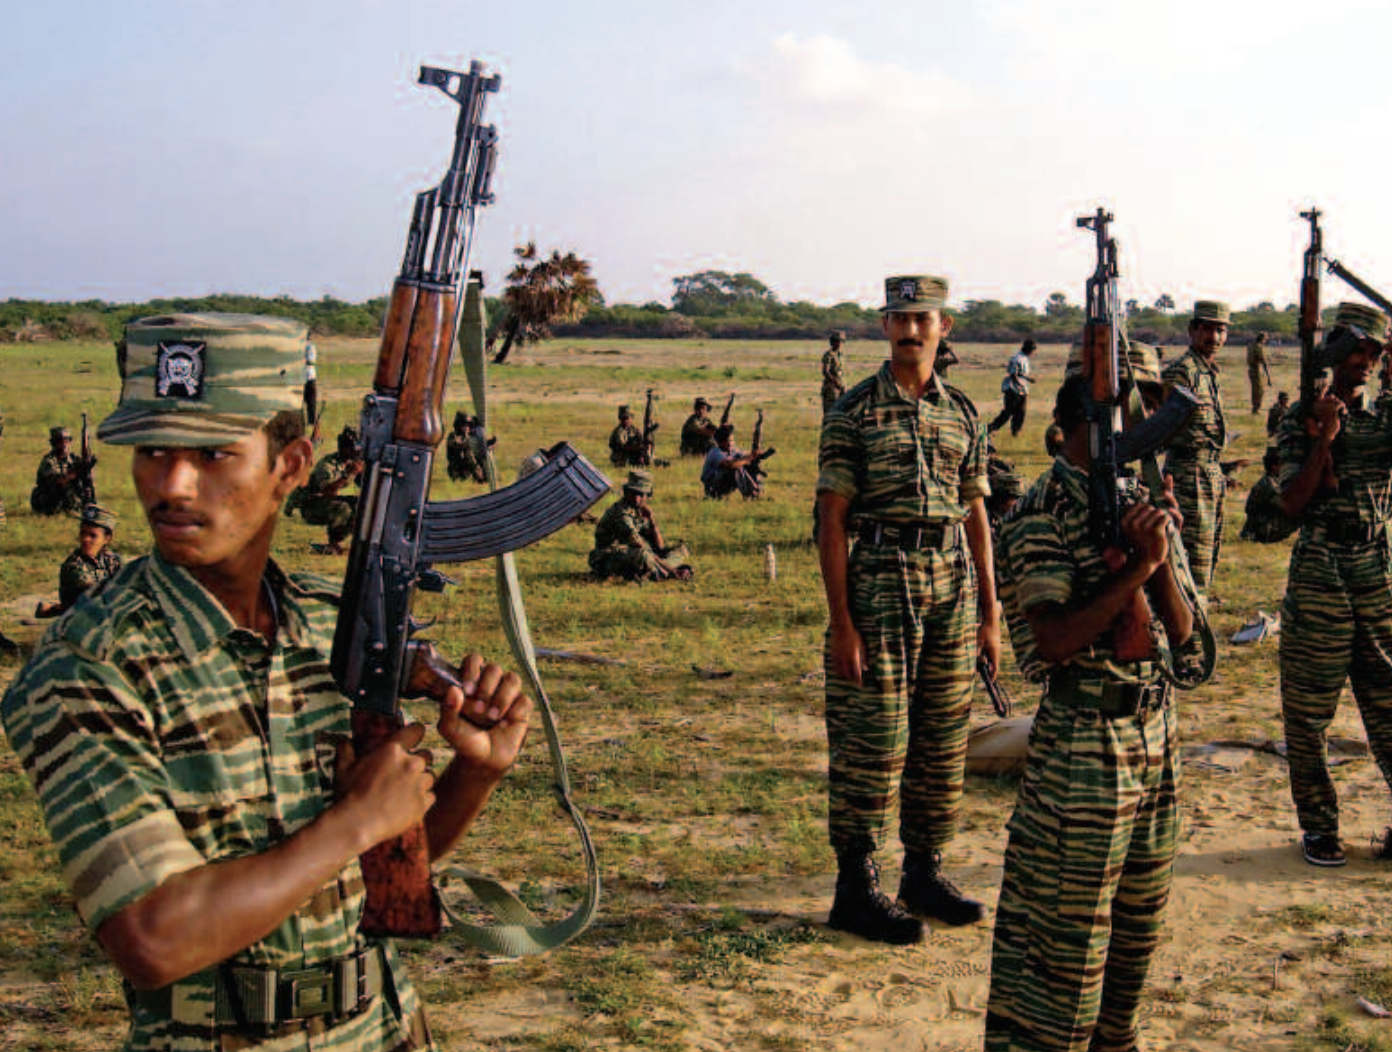
\includegraphics[width = 0.8\textwidth]{img/ltte}

\end{frame}
% ----------------------------------------------------

% ----------------------------------------------------
\begin{frame}
\frametitle{LTTE \& civilian governance}
\centering

\begin{minipage}{0.4\textwidth}\centering
  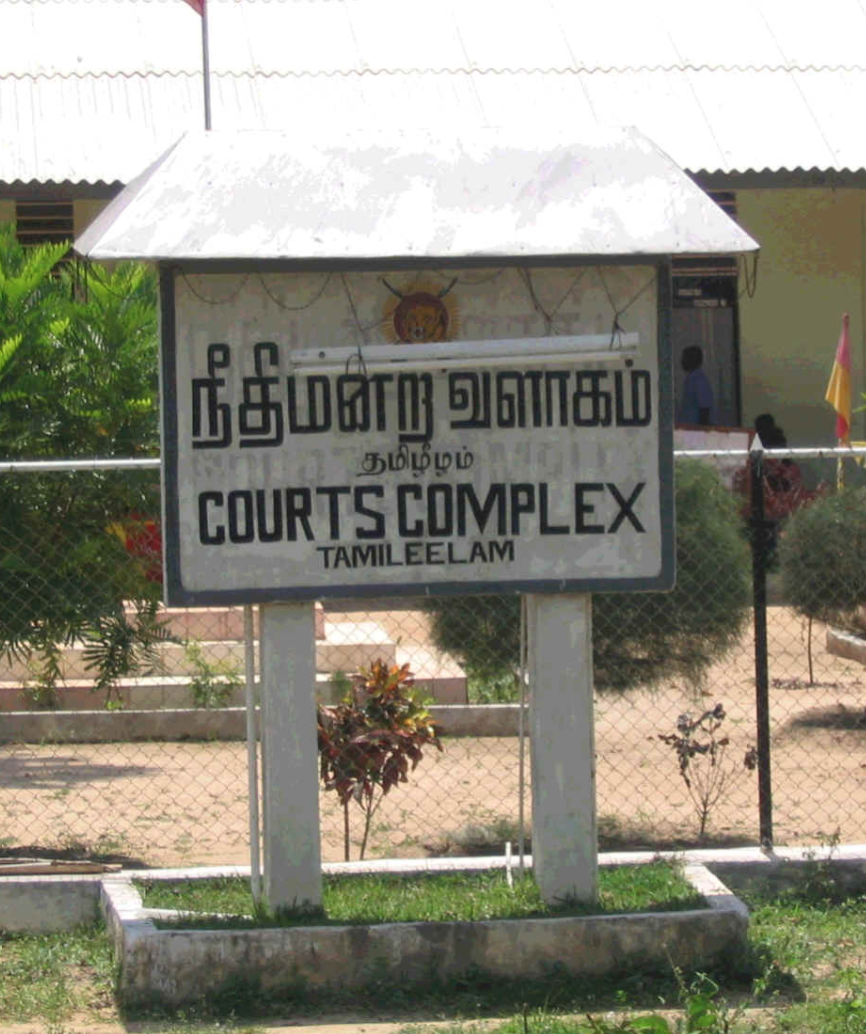
\includegraphics[width = 0.9\textwidth]{img/tamileelam_courts}
  \vfill
\end{minipage}\hfill
\begin{minipage}{0.59\textwidth}\centering
  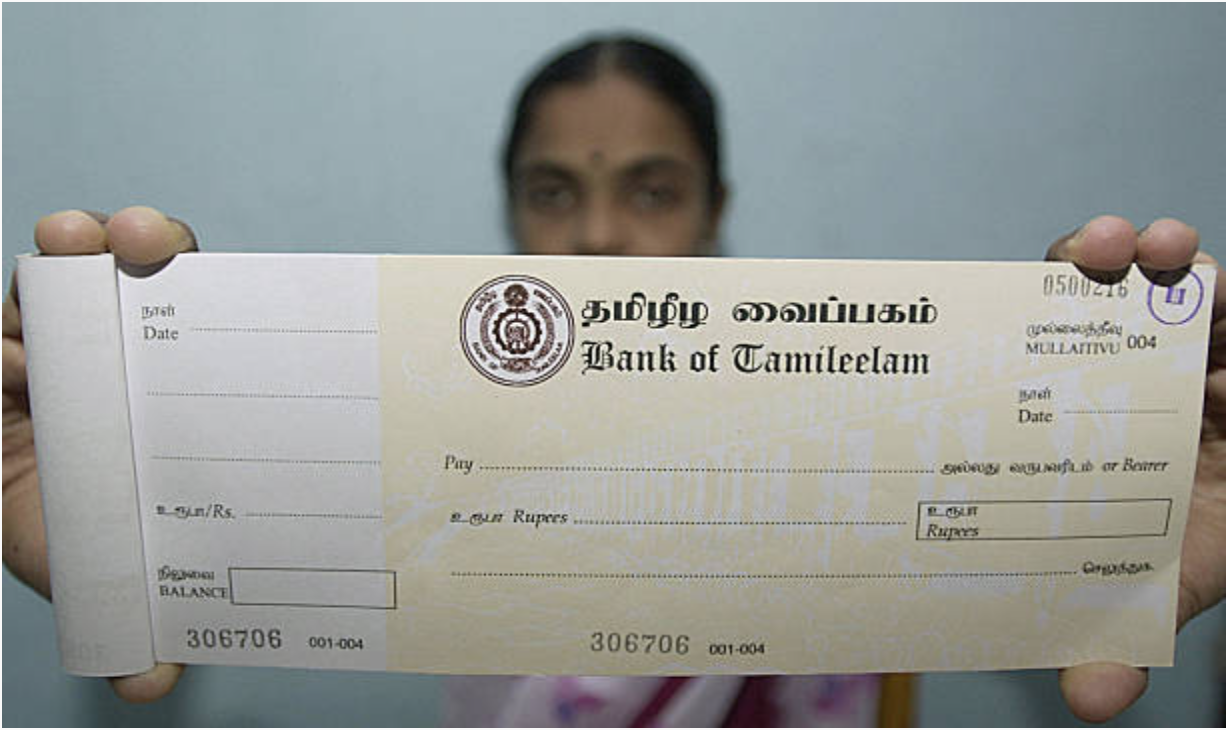
\includegraphics[width = \textwidth]{img/tamileelam_bank}\\
  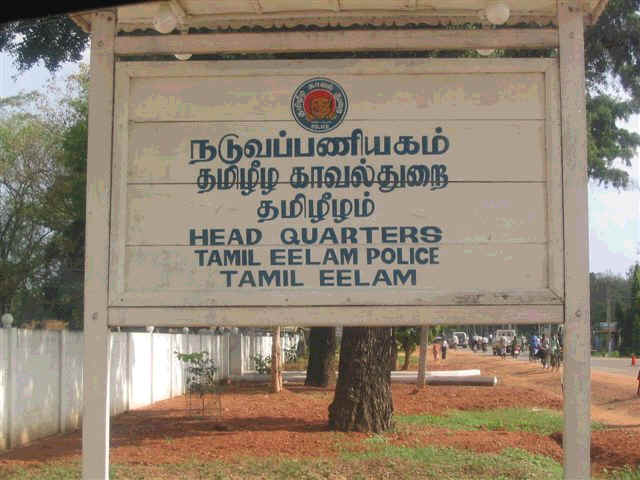
\includegraphics[width = \textwidth]{img/tamileelam_police}
\end{minipage}

\end{frame}
% ----------------------------------------------------

% ----------------------------------------------------
\begin{frame}
\frametitle{Understand governance}
\centering

\begin{itemize}
  \item<1-> A civil war is a conflict over control of territory and \textit{people}
  \begin{itemize}
    \item A crucial aspect: civilian collaboration
  \end{itemize}
  \item<2-> Civilians offer opportunities to the rebels (recruits, material support, information, etc) but can also defect to the enemy
  \item<3-> Rebel governance is developed to win over the support of the local population and disincentivize collaboration with the enemy
  \item<4-> Very dependent on territorial control: you can't obviously build banks or bureaucracies if you are a guerrilla group without firm territorial control
\end{itemize}

\end{frame}
% ----------------------------------------------------

% ----------------------------------------------------
\begin{frame}
\frametitle{Rebel governance}
\centering

\begin{itemize}
  \item But why?
\end{itemize}

\end{frame}
% ----------------------------------------------------

% ----------------------------------------------------
\begin{frame}
\frametitle{Greed perspective: Resources and control}
\centering

\begin{minipage}{0.6\textwidth}\centering
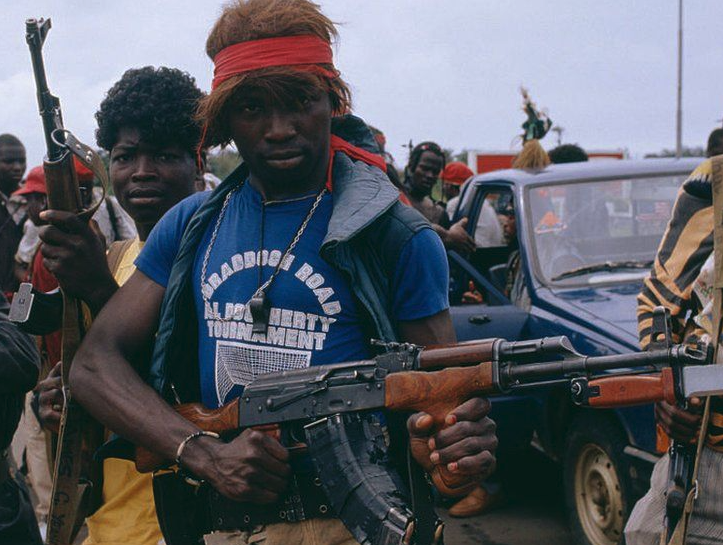
\includegraphics[width = 0.8\textwidth]{img/liberia}\\Liberia
\end{minipage}\hfill
\begin{minipage}{0.39\textwidth}\centering
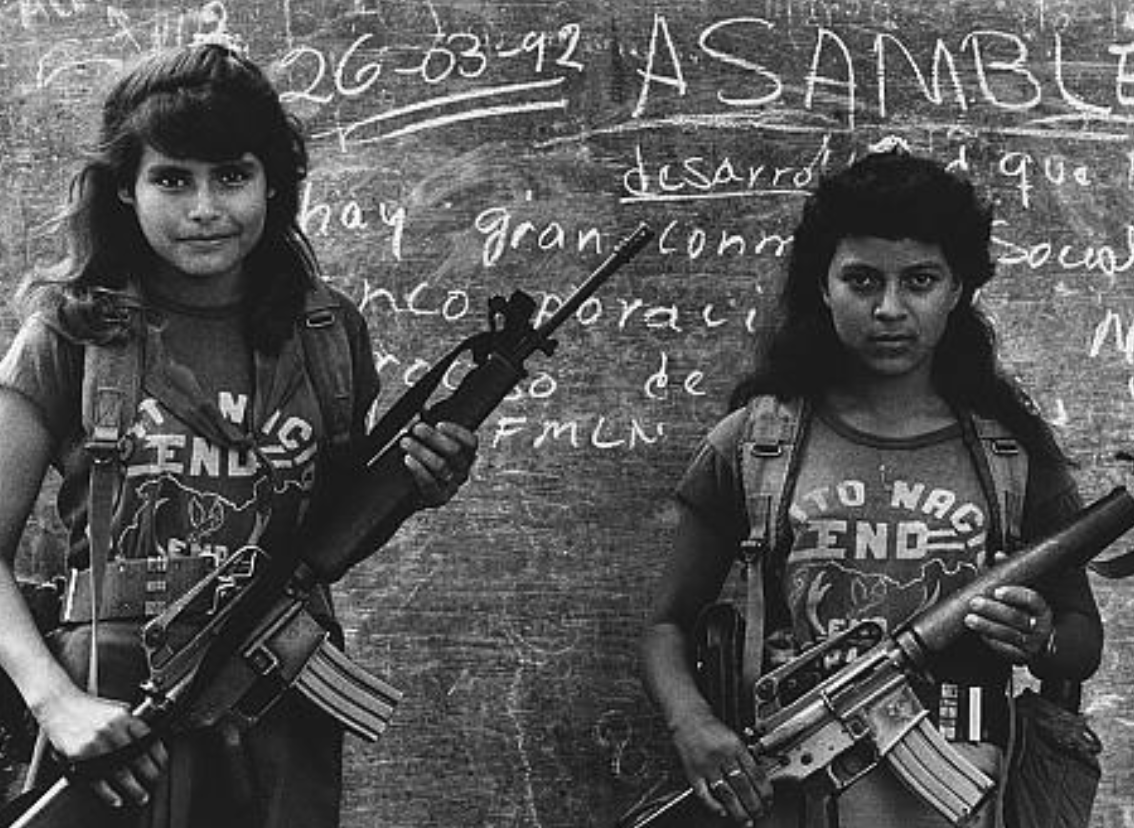
\includegraphics[width = 0.8\textwidth]{img/fmln}\\El Salvador
{\small Jeremy Weinstein (2007)}
\end{minipage}

\end{frame}
% ----------------------------------------------------

% ----------------------------------------------------
\begin{frame}
\frametitle{Greed perspective: Resources and control}
\centering

\begin{minipage}{0.6\textwidth}\centering
  \begin{itemize}[<+->]
    \item Why do some groups use violence while other restrain themselves?
    \item It depends on the initial conditions faced by rebel leaders:
    \item[1.] Do you have natural resources or foreign funding? No need for civilian cooperation, rule by the sword
    \item[2.] Do you need `social endowments'? You need to win `hearts and minds'
  \end{itemize}
\end{minipage}\hfill
\begin{minipage}{0.39\textwidth}\centering
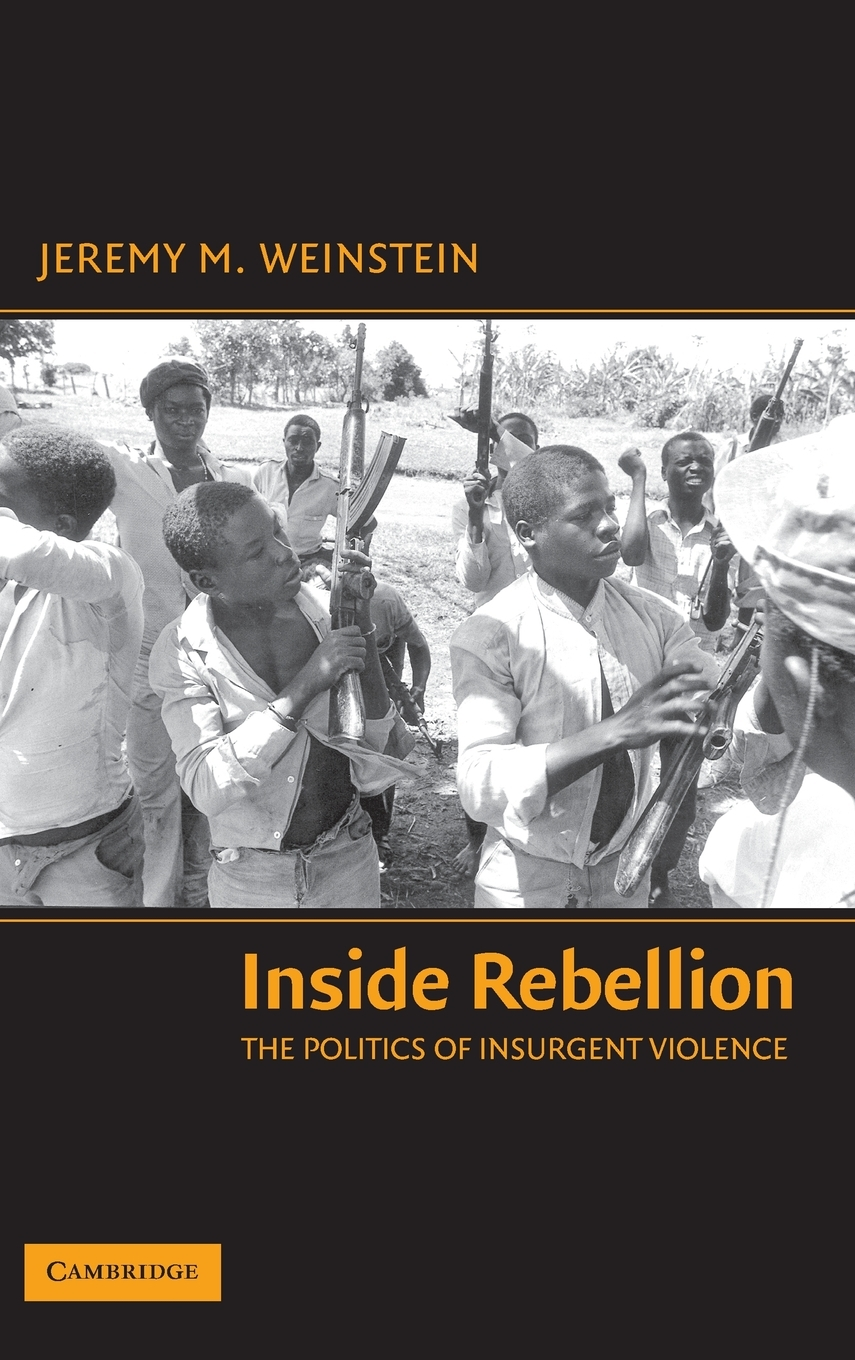
\includegraphics[width = 0.8\textwidth]{img/weinstein2007}\\
{\small Jeremy Weinstein (2007)}
\end{minipage}

\end{frame}
% ----------------------------------------------------

% ----------------------------------------------------
\begin{frame}
\frametitle{Resources and control: ISIS?}
\centering

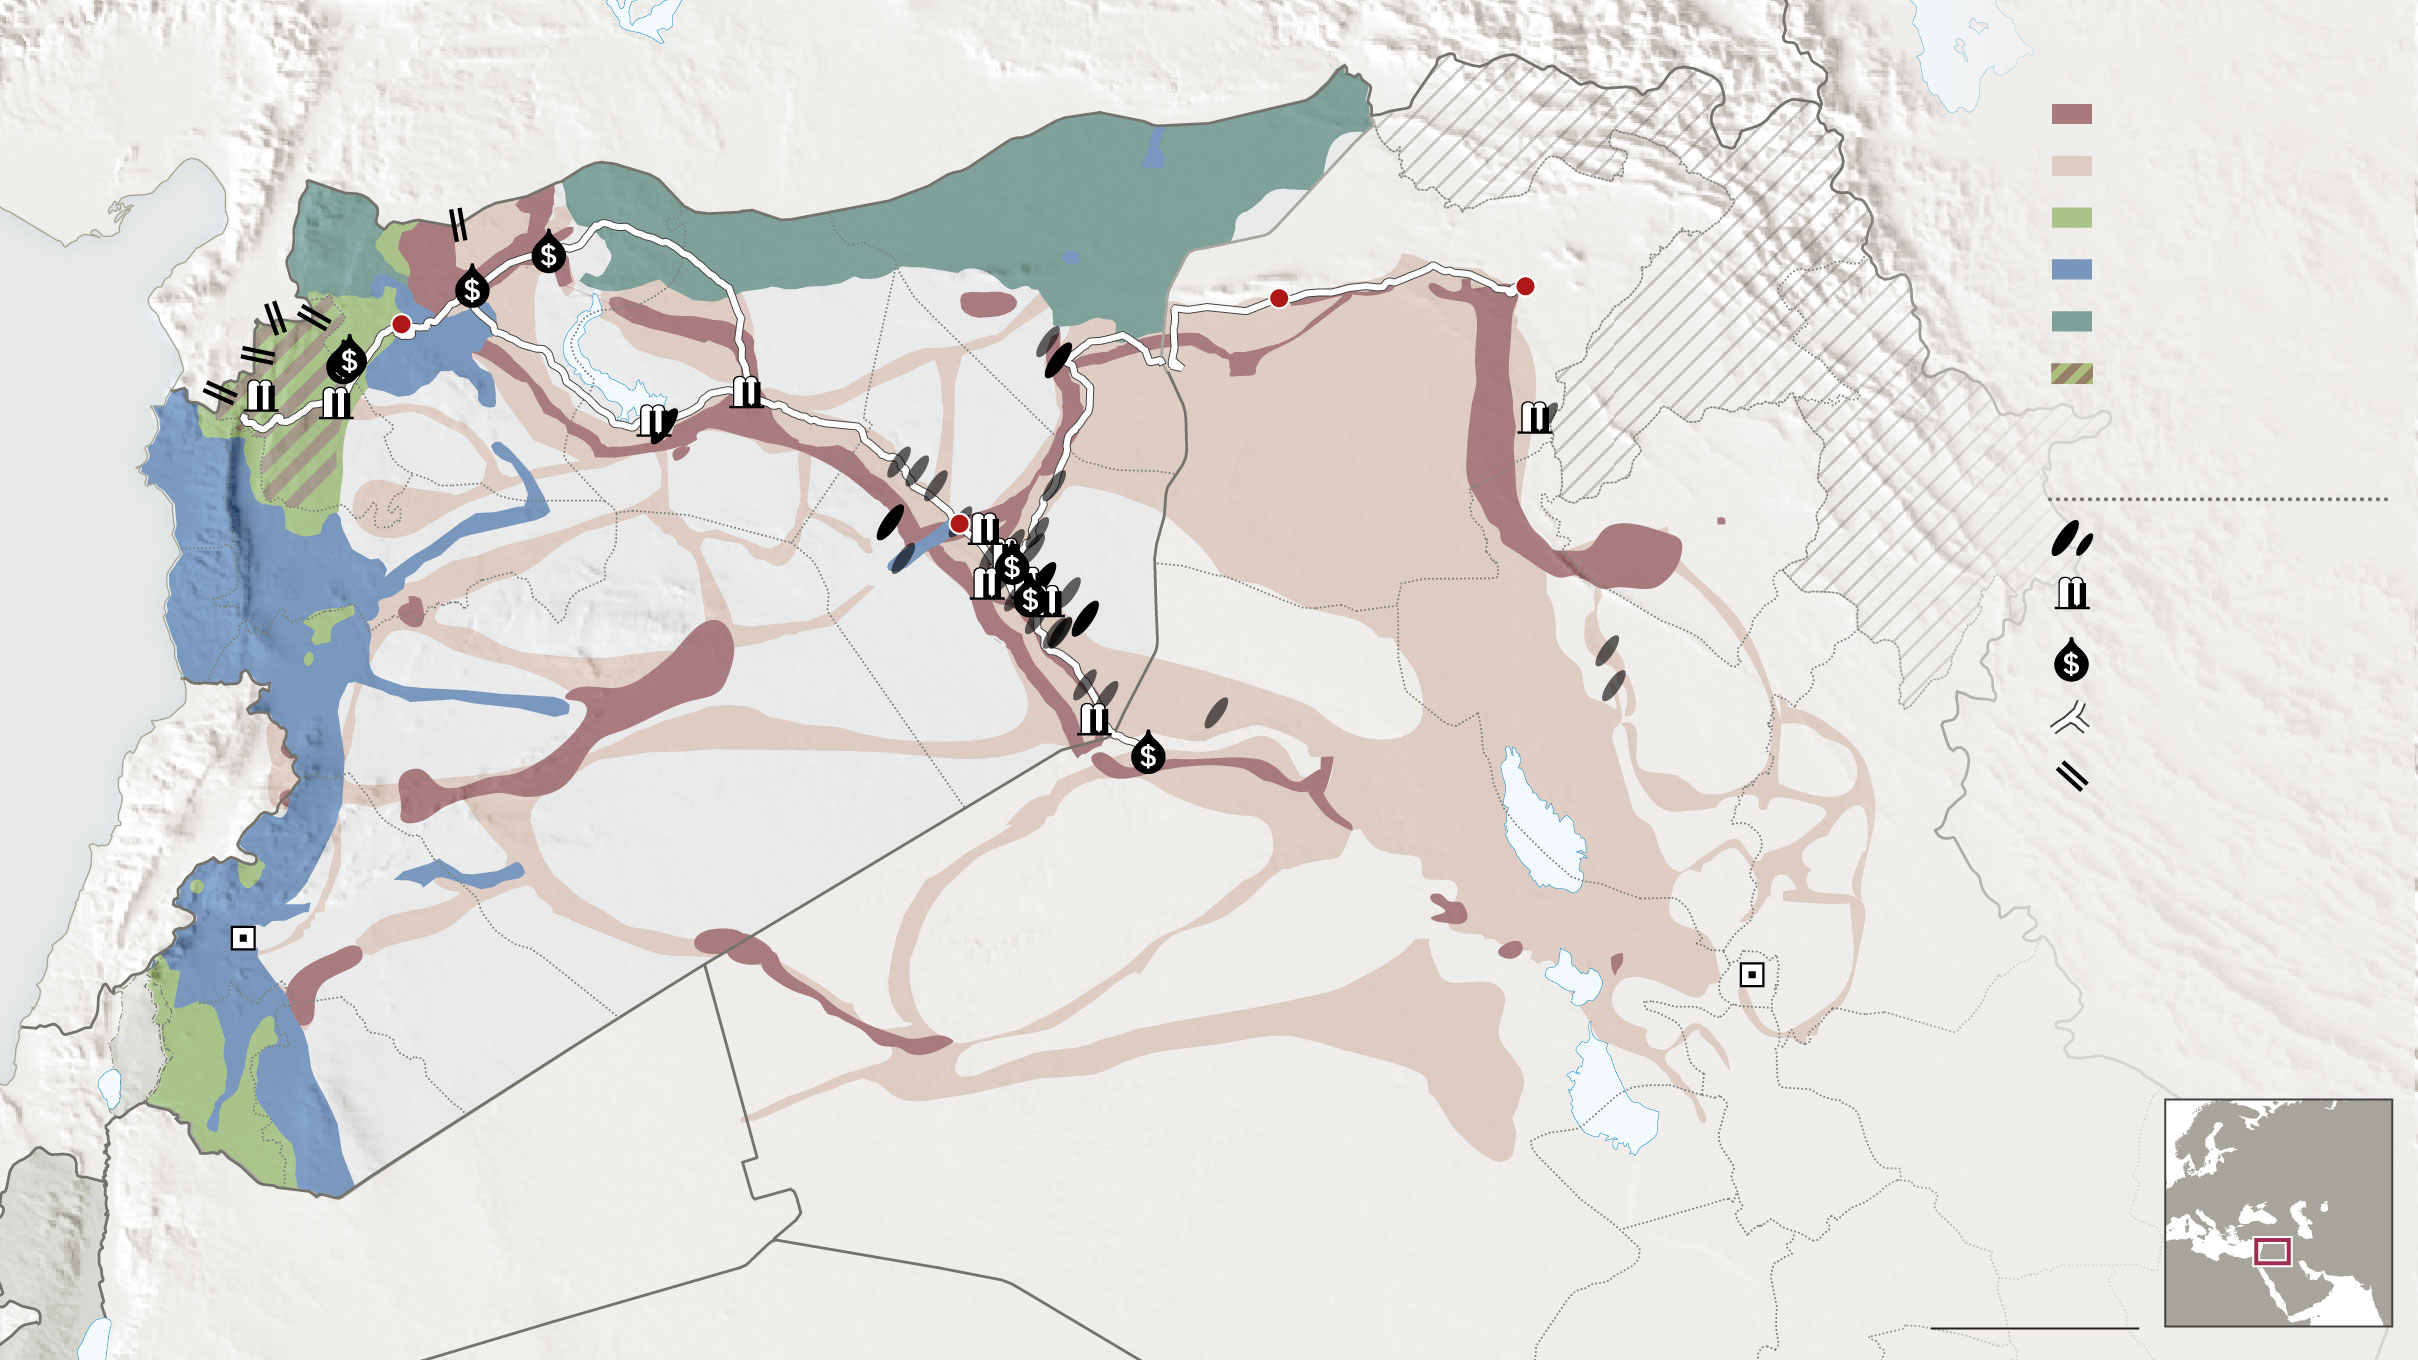
\includegraphics[width = \textwidth]{img/isis_syria_oil}

What would you expect from ISIS?

\end{frame}
% ----------------------------------------------------

% ----------------------------------------------------
\begin{frame}
\frametitle{Resources and control: ISIS?}
\centering

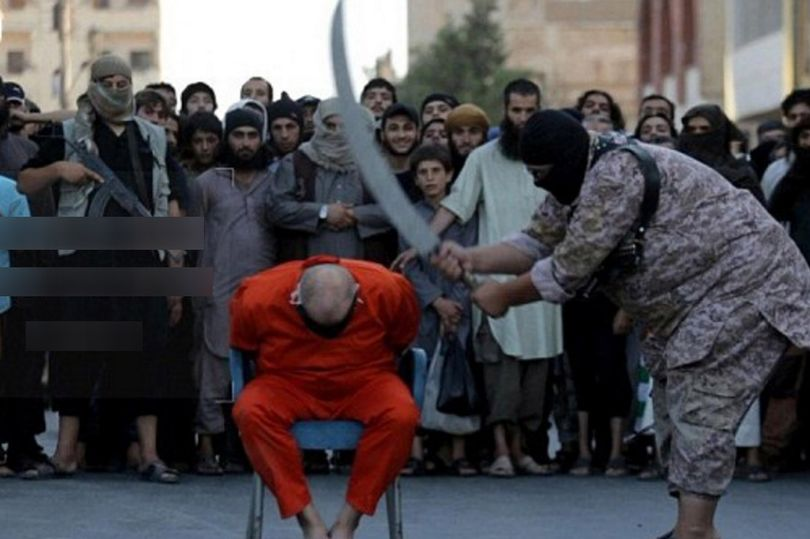
\includegraphics[width = 0.7\textwidth]{img/isis-raqqa}

\vspace{15pt}

ISIS public execution in Raqqa (Syrian Civil War)

\end{frame}
% ----------------------------------------------------

% ----------------------------------------------------
\begin{frame}
\frametitle{Resources and control: ISIS?}
\centering

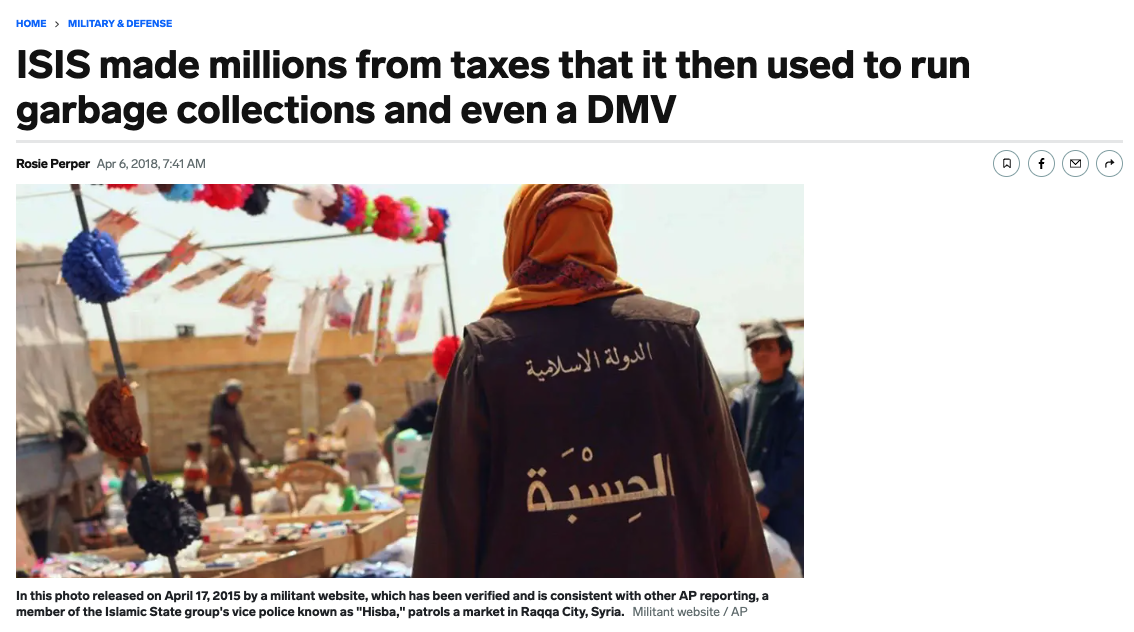
\includegraphics[width = \textwidth]{img/isis_taxing}

\end{frame}
% ----------------------------------------------------

% ----------------------------------------------------
\begin{frame}
\frametitle{Resources and control: ISIS?}
\centering

\begin{itemize}
  \item<1-> The role of ideology, not only material incentives
  \begin{itemize}
    \item Which also explains many other aspects of rebel governance
  \end{itemize}
  \item<2-> War pressures
  \begin{itemize}
    \item Similar to Tilly's state formation idea
  \end{itemize}
  \end{itemize}

\end{frame}
% ----------------------------------------------------


% ----------------------------------------------------
\begin{frame}
\frametitle{Understanding rebel governance}
\centering

\begin{itemize}[<+->]
  \item Violence alone is never enough, nor are just private, finantial incentives
  \item Given some degree of territorial control, some rebel governance usually exists
  \item But its \textbf{shape varies} a lot, which depends on several factors:
  \begin{itemize}
    \item Prewar cultural and political norms
    \item Problems that appear during the war
    \item Influence of local civilians
    \item Imitation of state symbols and practices
  \end{itemize}
  \item Some focus on economic production, health, education, some develop more participatory institutions, etc
\end{itemize}

\end{frame}
% ----------------------------------------------------

% ----------------------------------------------------
\begin{frame}
\frametitle{Understanding rebel governance}
\centering

\begin{minipage}{0.7\textwidth}\centering
  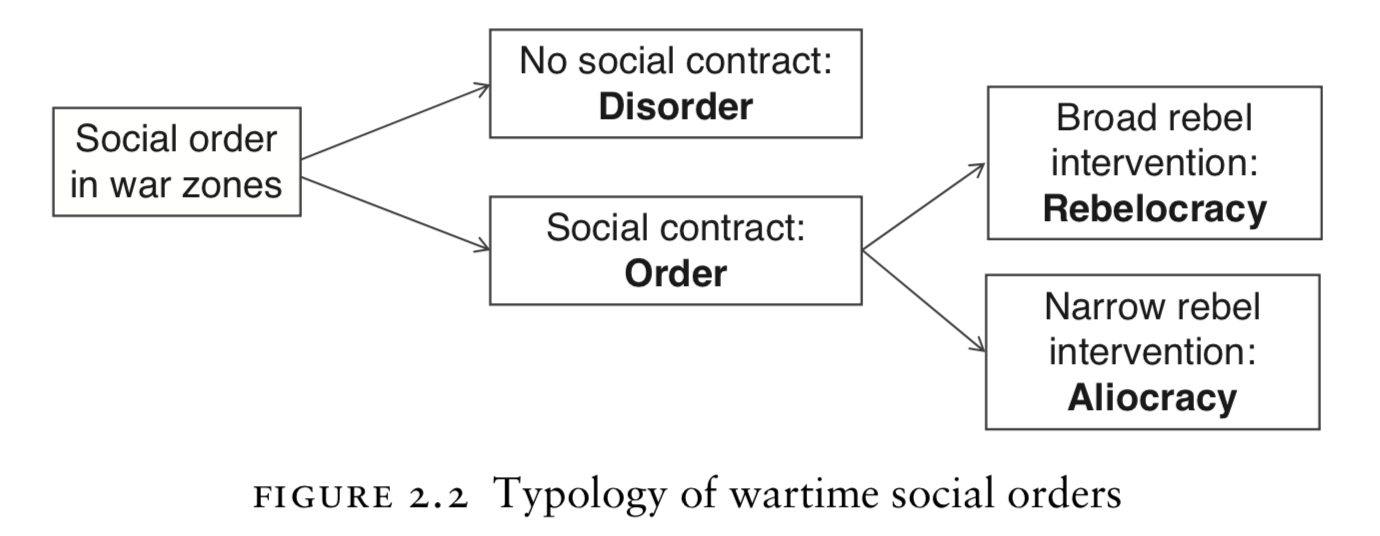
\includegraphics[width = \textwidth]{img/arjona_typology}\\\vspace{10pt}
  \begin{itemize}[<+->]
    \item {\small (\textit{Social contract}: expectations about behavior and enforcement, something like `laws')}
    \item Rebel groups try to mazimize territorial control and what they get out of it
    \item Therefore, they should prefer order to disorder, and more intervention (rebelocracy) than less (aliocracy)
  \end{itemize}
\end{minipage}\hfill
\begin{minipage}{0.29\textwidth}\centering
  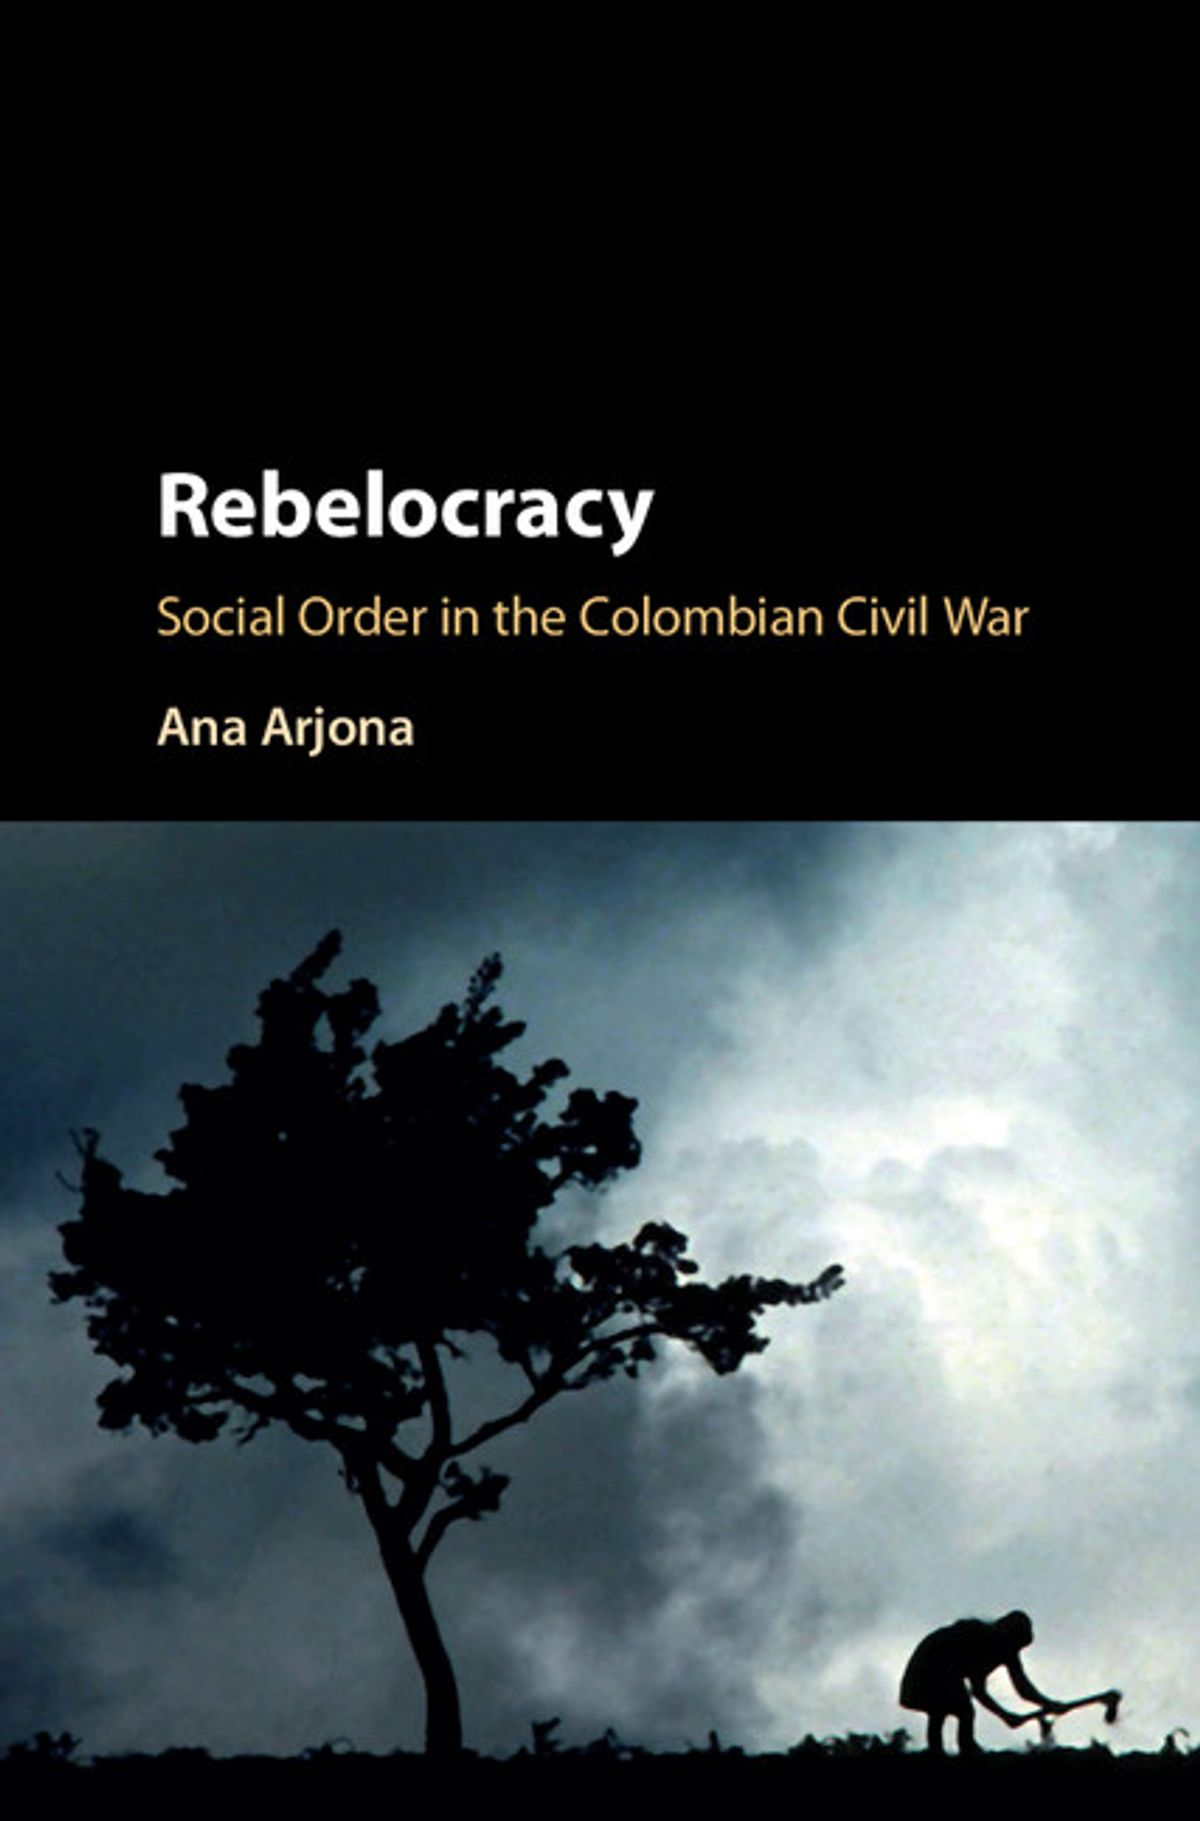
\includegraphics[width = 0.85\textwidth]{img/arjona_rebelocracy}\\
  {\small Ana Arjona (2017)}
\end{minipage}

\end{frame}
% ----------------------------------------------------

% ----------------------------------------------------
\begin{frame}
\frametitle{Understanding rebel governance}
\centering

% \begin{minipage}{0.7\textwidth}\centering
  \begin{itemize}[<+->]
    \item When does \textbf{order and rebelocracy} emerge? (i.e. when do rebel engage in extensive governance?)
    \item Depends on the rebels' time horizon and prewar local institutions
    \item[1.] If they have long-term expectationts (because of territorial competition, peace agreements, etc), rebels develop more comprehensive governance. Otherwise, there will be disorder
    \item[2.] Rebels prefer rebelocracy (replacing and controling all local social institutions), but this is not always possible
    \item[3.] This choice depends on the expectation of civilian resistance, which is shaped by preexisting institutions
    \item[4.] Areas where civilians retain control, rebels establish aliocracy: a form of indirect rule, controlling only the basics of security and taxation
  \end{itemize}
% \end{minipage}\hfill
% \begin{minipage}{0.29\textwidth}\centering
%   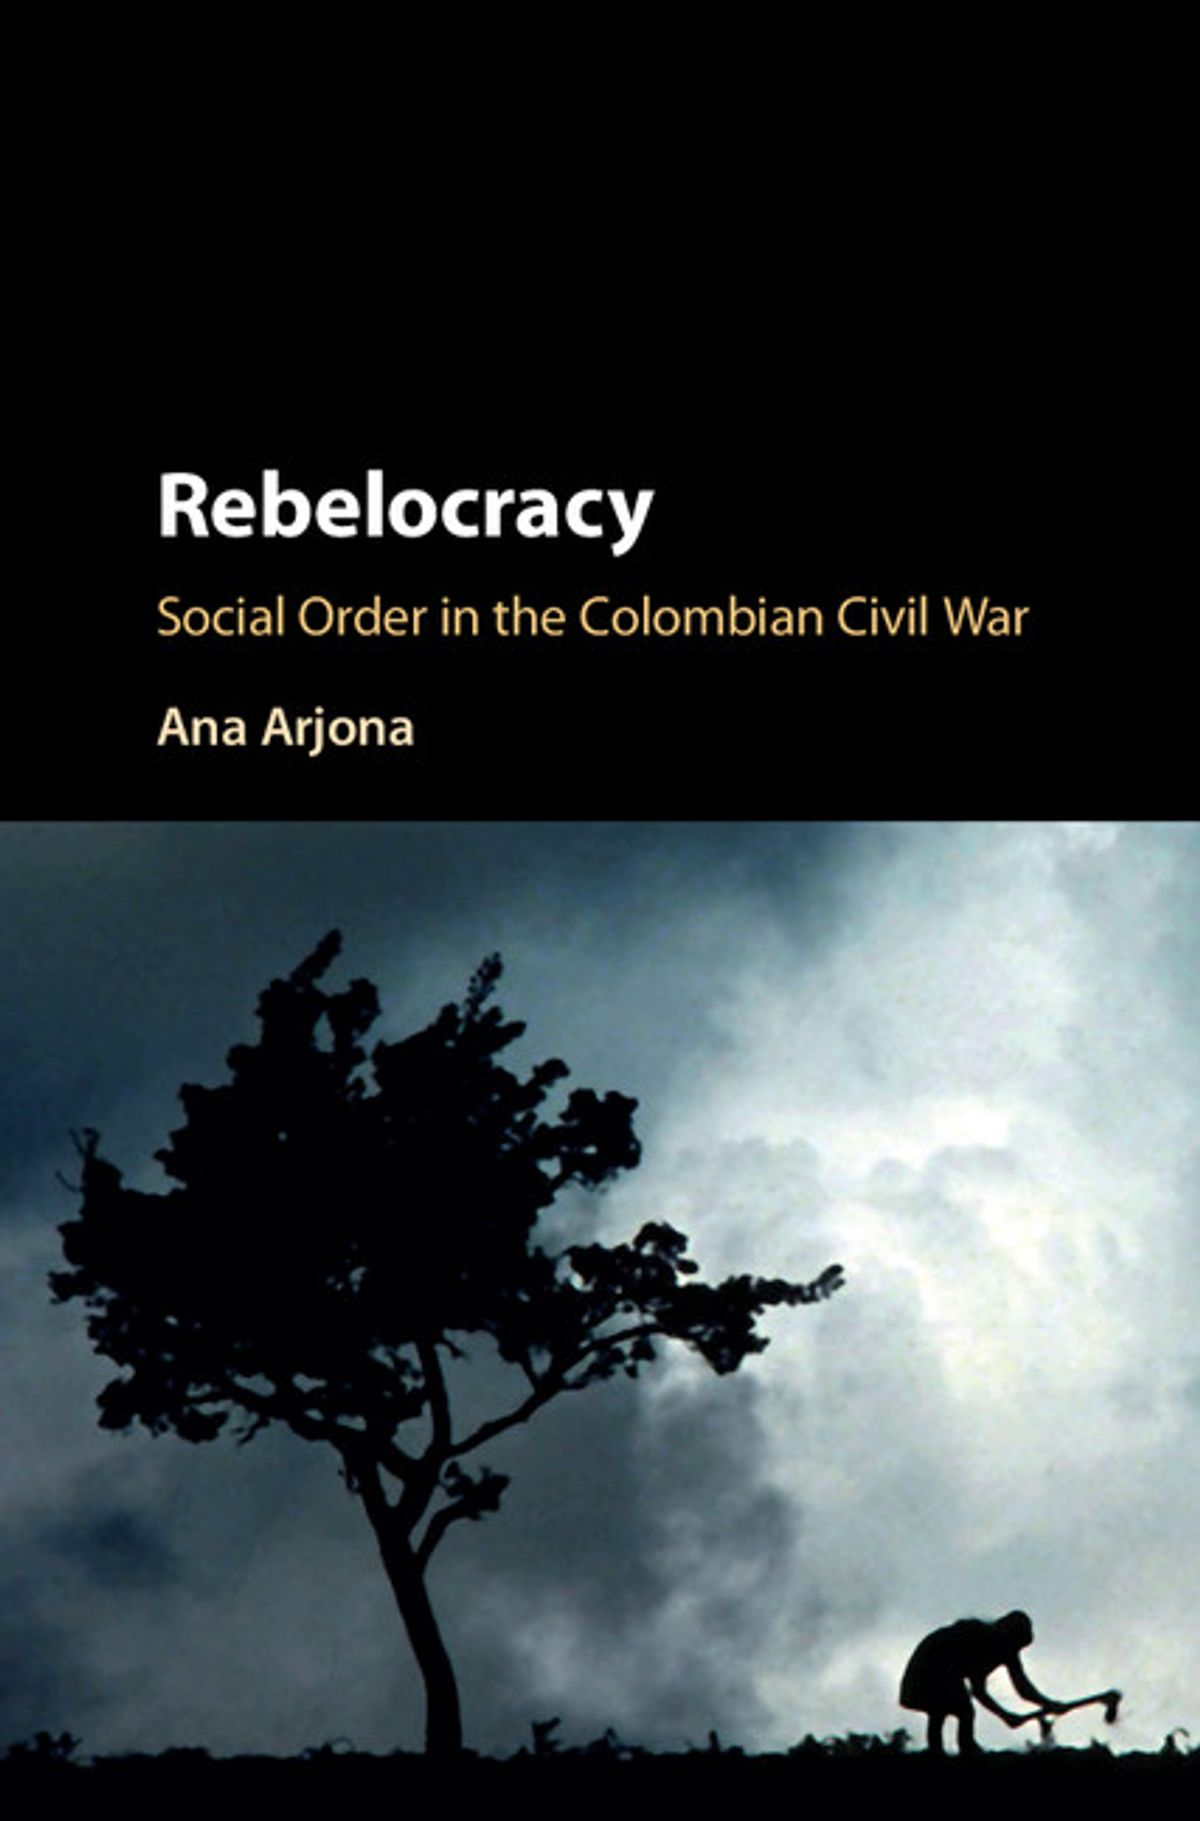
\includegraphics[width = 0.85\textwidth]{img/arjona_rebelocracy}\\
%   {\small Ana Arjona (2017)}
% \end{minipage}

% Arjona explains the variation in rebelocracy, aliocracy and disorder across time and space through the combination of armed groups’ time horizon and the quality of preexisting local institutions. Most rebels care about future outcomes and will seek to regulate private and public life broadly to induce civilian cooperation in areas where they have an ongoing presence. Particularly, they will establish mechanisms to adjudicate disputes, such as courts, as the administration of justice helps ‘armed groups centralize power and build an aura of legitimacy’ (56). Where preexisting institutions shape the capacity for civilians to collectively resist rebel rule and maintain control over civilian affairs, rebels will limit their influence and focus on basic elements of rule: that is, security and taxation. Under certain conditions, when rebels face internal indiscipline, external competition over territory or macro-changes in the war, such as peace negotiations, their focus on short-term goals will lead to disorder, or the absence of social contract in the communities.

\end{frame}
% ----------------------------------------------------

% ----------------------------------------------------
\begin{frame}
\frametitle{Civilian influence and resistance}
\centering

\begin{itemize}
  \item<1-> In brief, it works like a state-building process
  \item<2-> Some degree of opposition is always present, as in any political order
  \item<3-> Full resistance emerges when rebels try to fully replace existing social institutions that are valued locally
  \item<4-> In some cases, local organizations are able to challenge the monopoly of violence of rebels (self-defense etc) or influence local financing and taxation institutions
  \item<5-> Alliance formation (rebels, social sectors/orgs)
\end{itemize}

\end{frame}
% ----------------------------------------------------

% ----------------------------------------------------
\begin{frame}
\frametitle{Understanding rebel choices beyond governance}
\centering

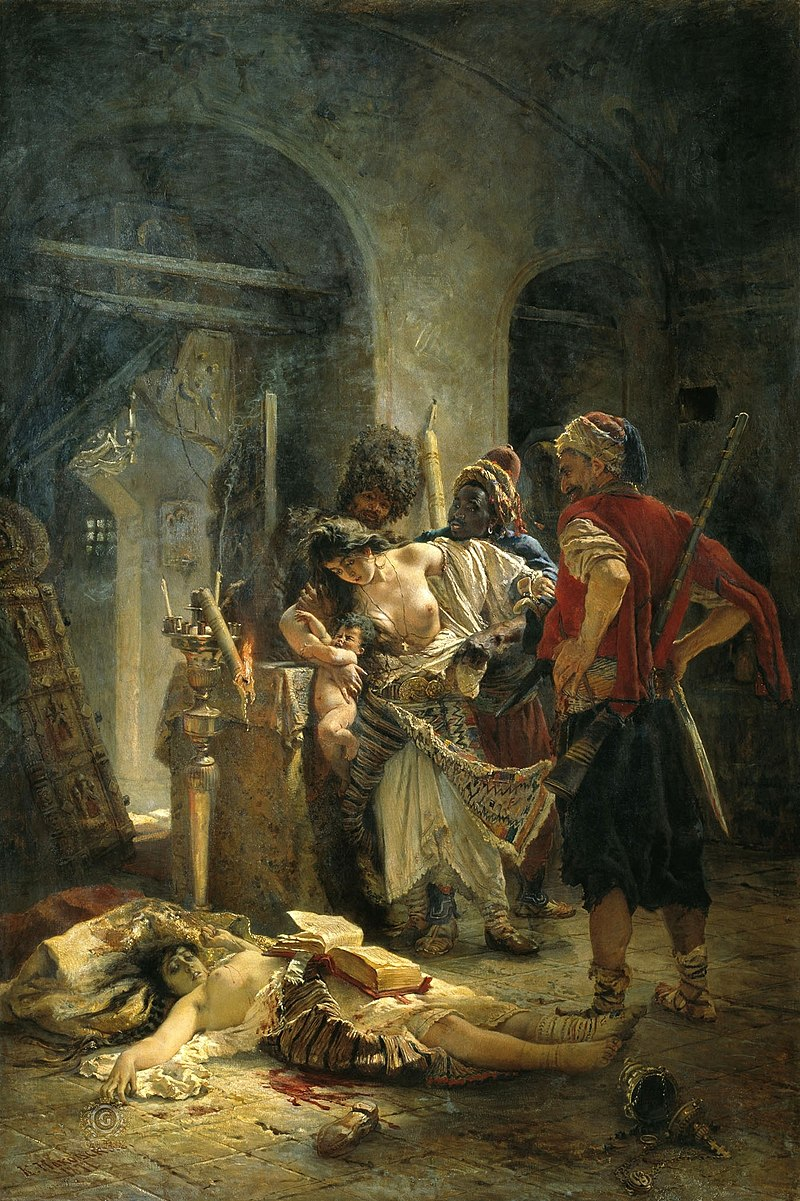
\includegraphics[width = 0.5\textwidth]{img/The_Bulgarian_martyresses}

\end{frame}
% ----------------------------------------------------

% ----------------------------------------------------
\begin{frame}<1-2>[label=rape]
\frametitle{Back to sexual violence}
\centering

\begin{itemize}
  \item<1-> What explains wartime sexual violence?
  \item[]
  \item<2-> Rape as collateral violence, opportunistic \& private reasons
  \item<3-> Rape as strategic violence
  \begin{itemize}
    \item Sexual violence offers organizational advantages related to warfare
  \end{itemize}
  \item<4-> Rape as \textit{practice}
  \begin{itemize}
    \item Socialization, organizational aspects, absence of restraint, etc
  \end{itemize}
\end{itemize}

\end{frame}
% ----------------------------------------------------

% ----------------------------------------------------
\begin{frame}
\frametitle{Back to sexual violence}
\centering

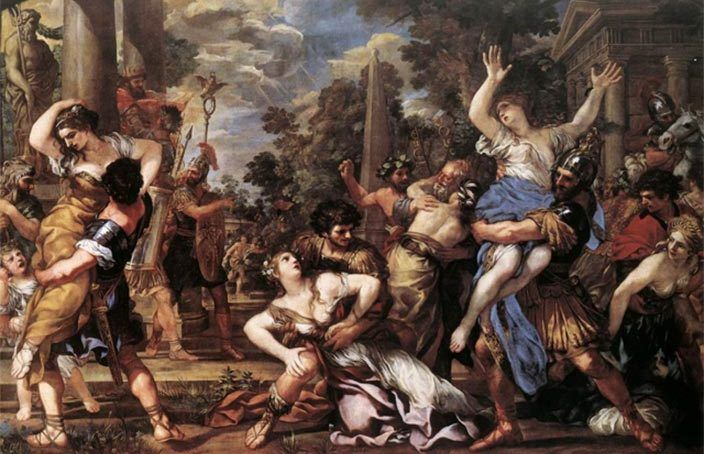
\includegraphics[width = 0.9\textwidth]{img/rape_history}

\end{frame}
% ----------------------------------------------------

% ----------------------------------------------------
\againframe<3>{rape}
% ----------------------------------------------------

% ----------------------------------------------------
\begin{frame}
\frametitle{Back to sexual violence}
\centering

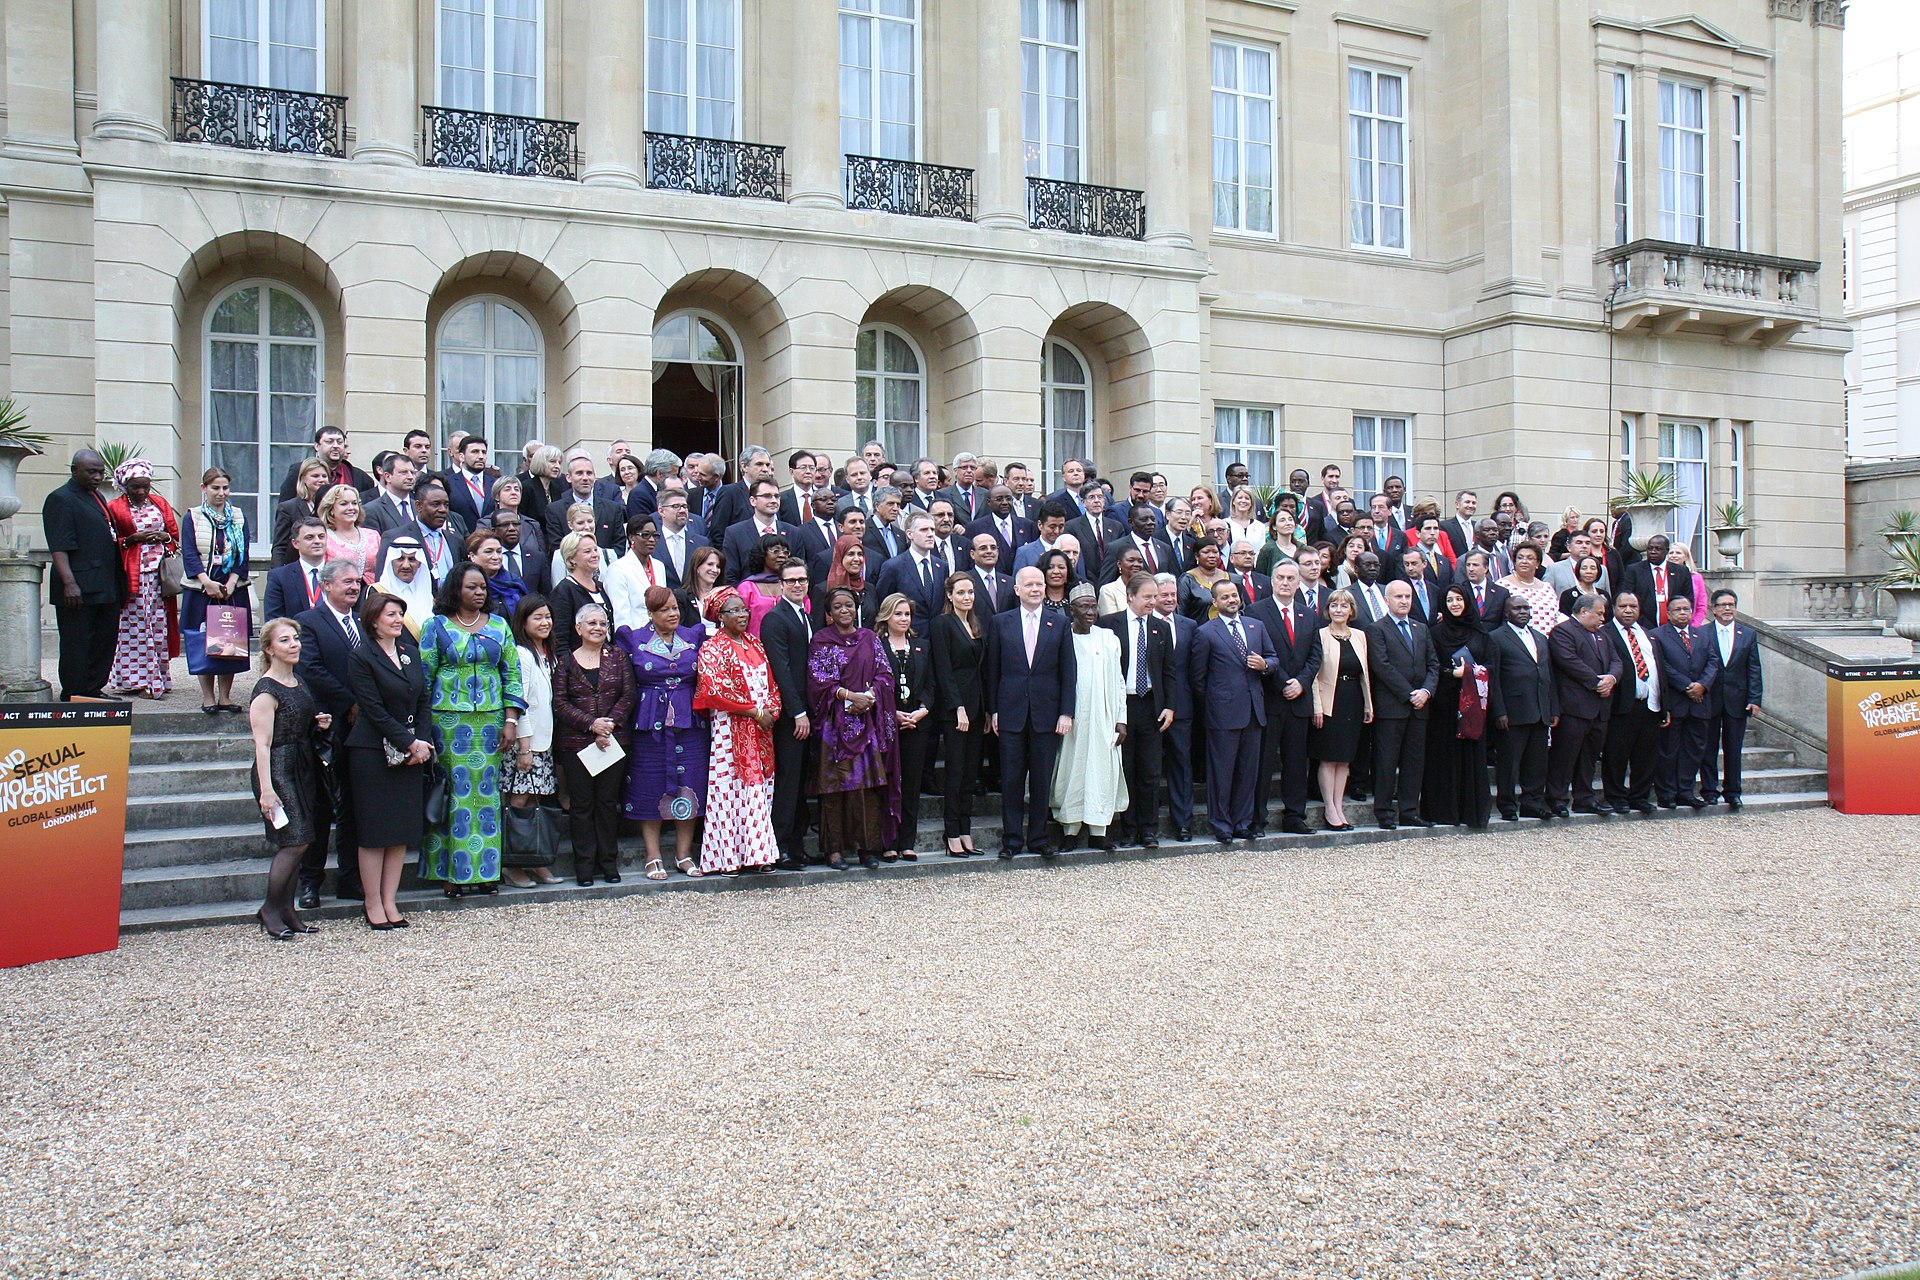
\includegraphics[width = \textwidth]{img/global_summit_rape}

Global Summit to End Sexual Violence in Conflict, 2014

\end{frame}
% ----------------------------------------------------

% ----------------------------------------------------
\againframe<4>{rape}
% ----------------------------------------------------

% ----------------------------------------------------
\begin{frame}
\frametitle{Back to sexual violence}
\centering

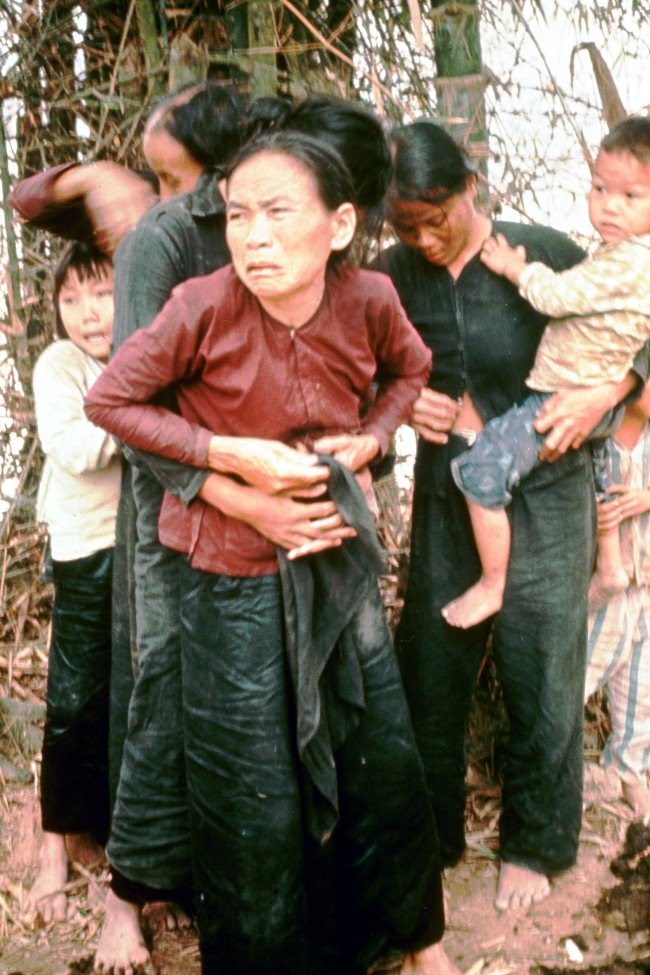
\includegraphics[width = 0.4\textwidth]{img/my_lai}

US troops in Vietnam, My Lai massacre (1968)

\end{frame}
% ----------------------------------------------------

% ----------------------------------------------------
\begin{frame}
\frametitle{Beyond civil wars: gangs}
\centering

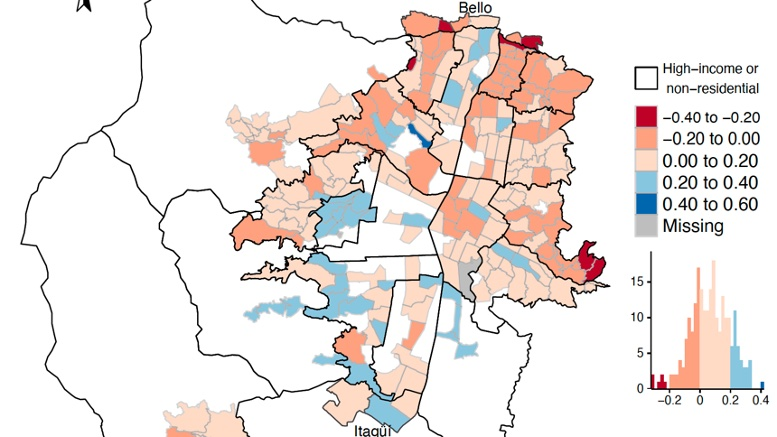
\includegraphics[width = 0.85\textwidth]{img/combo_governance_medelling}

Service provision by local gangs in Medellin (red means that the role of combo $>$ role of state)

\vspace{15pt}

{\footnotesize \textit{Source:} Chris Blattman et al)}

\end{frame}
% ----------------------------------------------------

% ----------------------------------------------------
\begin{frame}
\frametitle{Beyond civil wars: gangs}
\centering

% CHRIS BLATTMAN:
% https://twitter.com/cblatts/status/1311474471874760704

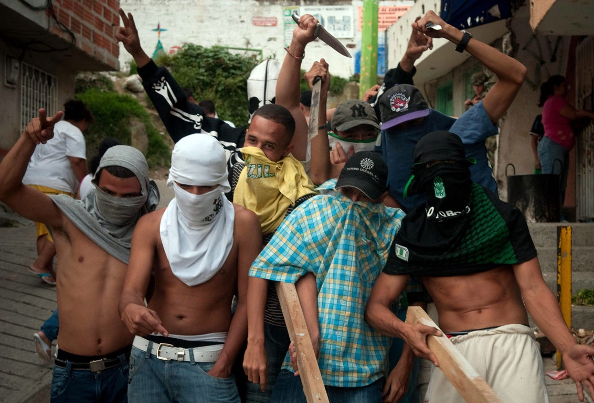
\includegraphics[width = 0.8\textwidth]{img/combo}

\vspace{15pt}

`Combo' members in Colombia

\end{frame}
% ----------------------------------------------------

% ----------------------------------------------------
\begin{frame}
\frametitle{Beyond civil wars: gangs}
\centering

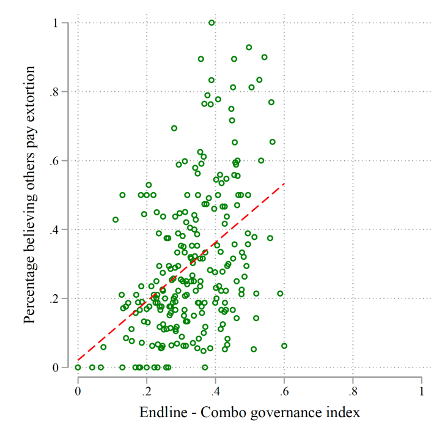
\includegraphics[width = 0.5\textwidth]{img/combo_gov_index_taxation}

Gangs governance: it will be related to taxes/extortion, but it's also a choice

\vspace{15pt}


\end{frame}
% ----------------------------------------------------

% ----------------------------------------------------
\begin{frame}
\frametitle{Beyond civil wars: gangs}
\centering

\begin{itemize}
  \item Where should we see combos more likely to engage in governance?
\end{itemize}

\vspace{15pt}


\end{frame}
% ----------------------------------------------------

% ----------------------------------------------------
\begin{frame}
\frametitle{Beyond civil wars: gangs}
\centering

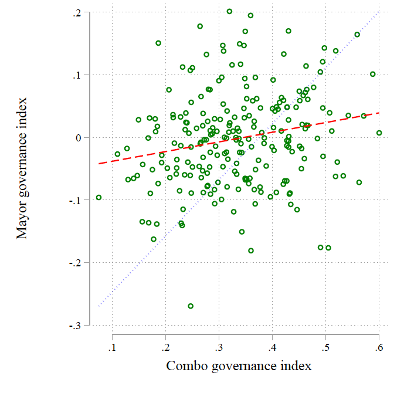
\includegraphics[width = 0.5\textwidth]{img/combo_mayor_gov_index}

Gangs governance and local government, they overlap

\vspace{15pt}

\end{frame}
% ----------------------------------------------------


\end{document}
